\documentclass[5p,letterpaper]{article}
\usepackage{lipsum}
\usepackage{caption}
\usepackage[utf8]{inputenc}
\usepackage{setspace}
\usepackage[T1]{fontenc}
\usepackage[spanish]{babel}
\usepackage{multicol}
\usepackage{latexsym,amsmath,amssymb,amsfonts}
\usepackage{bm}
\usepackage{physics}
\usepackage{graphicx}
\usepackage{wrapfig}
\usepackage{multirow}
\usepackage{subcaption}
\usepackage{enumerate}
\usepackage{float}
\usepackage{listings}
\usepackage{xcolor}
\usepackage{fancyhdr}
\usepackage{braket}
\usepackage{hyperref}
\usepackage{dsfont}
\parindent = 6mm
\newcommand{\symd}{\triangle}
\usepackage{derivative}
\usepackage{comment}
\usepackage{tensor}
\usepackage{setspace}
\usepackage{mathtools} 
\usepackage{authblk}
%\usepackage[backend = biber]{biblatex}
\decimalpoint
% \usepackage[left=2.54cm,right=2.54cm,top=2.54cm,bottom=2.54cm]{geometry}
\usepackage[left=2 cm,top=2.0cm,right=2cm,bottom=3cm]{geometry}
\decimalpoint
\hypersetup{
    colorlinks=true,
    linkcolor=blue,
    filecolor=magenta,      
    urlcolor=cyan,
    pdftitle={Overleaf Example},
    pdfpagemode=FullScreen,
    }

% Title info
\title{\textbf{Laboratorio 04 — Telescopio y microscopio}}
\author{
  Jose Manuel Padilla Pérez \\
  Juan Manuel Grisales Martínez \\
  Martina García Mejía
}
\date{Septiembre 2025}
\begin{document}

\maketitle

\section{Objetivos}

Los objetivos de este laboratorio consisten en comprender el funcionamiento del telescopio refractor y el microscopio, además de comprender el funcionamiento de los diafragmas y las pupilas. Sumado a esto, corroborar que los cálculos teóricos coincidan con los experimentales.

\section{Metodología}

Para este laboratorio se utilizaron dos lentes con soporte las cuales tenían 50 mm y 30 mm de distancia focal respectivamente, utilizando el modelo de telescopio refractor de Kepler y el modelo de microscopio, se obtuvieron configuraciones para poder determinar el aumento de las imágenes para los dos sistemas, y cómo se ve afectado el microscopio con la pupila y/o diafragma. El primer montaje del telescopio consistió en poner las lentes a una distancia de 80 mm una de la otra debido a que es la suma de sus distancias focales. El segundo montaje fue sumarle una separación de 16 cm entre las lentes para tener la distancia efectiva del microscopio y luego ubicar los diafragmas para observar cuáles son los cambios sufridos en la imagen.

\section{Respuestas}

\subsection{Configuración del telescopio}
Para este apartado del laboratorio se emplearon las lentes, posicionándolas de tal forma en que la distancia entre ellas fuera la suma de las distancias focales de las lentes, obteniendo una separación de 8 cm.

Para la estimación del aumento experimental realizamos la comparación de imágenes, tomamos una foto sin el telescopio y otra en la misma posición con el mismo, como se observa en las figuras 1 y 2 la diferencia de tamaños, así sacamos el aumento dividiendo el tamaño de la imagen con el tamaño del objeto, lo cual nos dio un valor de: $m_{exp} = 1.36$.

\begin{figure}[H]
    \begin{minipage}{0.48\textwidth} % Ajusta el ancho según necesites
        \centering
        \includegraphics[width=\linewidth]{SSP_12.NEF}
        \caption{Imagen sin telescopio}
        \label{fig:imagen1}
    \end{minipage}
    \hfill % Espacio entre las imágenes
    \begin{minipage}{0.48\textwidth} % Ajusta el ancho según necesites
        \centering
        \includegraphics[width=\linewidth]{SSP_13.NEF}
        \caption{Imagen con telescopio}
        \label{fig:imagen2}
    \end{minipage}
\end{figure}

Utilizando la configuración Kepleriana de los telescopios podemos hallar el aumento nominal teórico para nuestro experimento, obteniéndolo de la relación entre la distancia focal del objetivo y la distancia focal del ocular:

\begin{equation}
    m_{nom}= -\frac{f_{ob}}{f_{oc}}
\end{equation}

Para nuestro caso sería:
\begin{equation}
    m_{nom}=-\frac{-50mm}{30mm} \approx 1.6
\end{equation}

De esta forma obtenemos que respecto al valor teórico tenemos una discrepancia del $22.15\%$. Este valor puede atribuirse a errores en la configuración experimental, como una separación entre lentes distinta a la distancia óptima $L =f_1 +f_2=80 mm$, lo que altera el aumento efectivo. Además, las aberraciones ópticas (esférica y cromática) en lentes simples distorsionan la imagen, y el enfoque no ajustado al infinito (dado que el objeto estaba en distancias finitas) reduce el aumento respecto al teórico. Finalmente, incertidumbres en la medición de tamaños aparentes en las fotografías y una posible identificación incorrecta de los roles de las lentes contribuyen a la diferencia observada.

\subsection{Configuración del microscopio}

Para el montaje del microscopio se utilizaron dos lentes positivas con distancias focales de $f_{ob}=50 \ \text{mm}$ (objetivo) y $f_{oc}=30 \ \text{mm}$ (ocular). La separación entre ellas se fijó en $L=16 \ \text{cm}$, de modo que el objetivo formara una imagen intermedia real y aumentada que pudiera ser observada por el ocular.

Con el fin de estimar el aumento experimental del sistema se empleó como objeto una lámina con franjas regulares cuya densidad aproximada era de $5 \ \text{líneas/mm}$, es decir, una separación real entre líneas de $0.2 \ \text{mm}$. Al observar la imagen a través del microscopio y registrarla con la cámara, se determinó que la separación aparente entre líneas se amplificó hasta aproximadamente $1 \ \text{línea/cm}$, lo que equivale a un espaciamiento de $10 \ \text{mm}$ en la imagen. De esta forma, el aumento lineal experimental del microscopio puede escribirse como
\begin{equation}
    m_{exp} = \frac{10 \ \text{mm}}{0.2 \ \text{mm}} = 50.
\end{equation}

El aumento nominal teórico del microscopio se determina como el producto entre el aumento lateral del objetivo y la amplificación angular del ocular. Para el objetivo, utilizando la aproximación de longitud de tubo $L$, se tiene:
\begin{equation}
    m_{ob} \approx \frac{L}{f_{ob}} = \frac{160 \ \text{mm}}{50 \ \text{mm}} = 3.2.
\end{equation}

Para el ocular, el aumento angular se expresa como
\begin{equation}
    M_{oc} = \frac{25 \ \text{cm}}{f_{oc}} = \frac{250 \ \text{mm}}{30 \ \text{mm}} \approx 8.3.
\end{equation}

El aumento nominal total resulta entonces:
\begin{equation}
    M_{nom} = m_{ob} \cdot M_{oc} \approx 3.2 \times 8.3 \approx 26.6.
\end{equation}

Comparando ambos resultados, el valor experimental $m_{exp}=50$ es casi el doble del aumento nominal esperado $M_{nom}\approx 26.6$. Esta diferencia puede atribuirse a factores experimentales como la dificultad para fijar con precisión la separación $L$, aberraciones de las lentes utilizadas, la referencia fotográfica no perfectamente coplanar con el objeto, así como a las limitaciones al medir las separaciones en la imagen. A pesar de ello, los órdenes de magnitud son consistentes y confirman que el microscopio construido amplifica de manera significativa un objeto de dimensiones micrométricas.



\subsection{Acople pupilas y sistemas}
El acople que se realiza utilizando las pupilas del ojo para el sistema, bien sea telescopio o microscopio, se tiene que al estar correctamente posicionados (para este caso) así obteniendo una imagen con buena definición. De esta forma, se puede notar que la distancia para el sistema entre las dos lentes es la correcta, pero no solo se debe tener eso para una correcta visualización de la imagen, sino que al utilizar el ojo se debe colocar a una distancia prudente, la cual, para el caso del laboratorio, se usa la distancia focal del segundo lente o ocular. \\
Por último, cabe aclarar que dentro de un rango la imagen conserva la calidad suficiente y al alejarse o acercarse, el campo de visión se incrementa o se reduce dependiendo de la posición del ojo, pudiendo aproximar el sistema a una clase de lupa con un mayor aumento.

\subsection{Posiciones de diafragmas}

Para los diafragmas se utilizaron las siguientes posiciones como se aprecia en la imagen:
\begin{figure} [H]
    \centering
    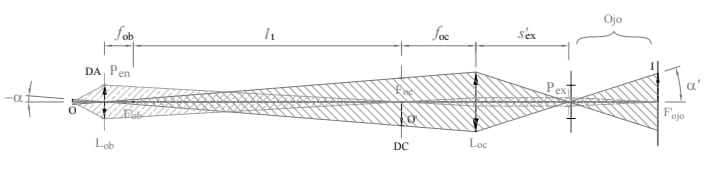
\includegraphics[width=0.5\linewidth]{Imagenes/optica diafragma lab 04.jpeg}
    \caption{Diagrama del sistema óptico creado para un microscopio}
    \label{fig:placeholder}
\end{figure}
Así colocamos el diafragma de apertura muy cercano a la lente primaria/objetivo y el diafragma de campo en la distancia focal de la lente auxiliar u ocular, viendo que en las siguientes imágenes:
\begin{figure}[H]
    \centering
    \includegraphics[width=0.5\linewidth]{}
    \caption{Imagen sin diafragma}
    \label{fig:placeholder}
\end{figure}
\begin{figure}[H]
    \centering
    \includegraphics[width=0.5\linewidth]{}
    \caption{Imagen diafragma DC<DA}
    \label{fig:placeholder}
\end{figure}
\begin{figure}[H]
    \centering
    \includegraphics[width=0.5\linewidth]{}
    \caption{Imagen diafragma DC>DA}
    \label{fig:placeholder}
\end{figure}
Se puede ver cómo al tener un diafrágma campo menor $(DC<DA)$ la cantidad de información del objeto se reduce, mientras que al usar el diafragma de apertura más pequeño $(DC>DA)$ la iluminación y el contraste pueden verse afectados disminuyendo, pero para ciertos criterios, la reducción del nivel de iluminación es necesaria para poder observar lo que se requiere en algunos puntos del sistema.

\subsection{Conclusiones}

Las conclusiones del experimento permitieron validar parcialmente el modelo teórico del telescopio refractor, aunque se observó una discrepancia del $22.15\%$ entre el aumento estimado experimentalmente ($A_{exp} =1.36$) y el aumento nominal teórico ($A_{nom}=1.6$). Esta diferencia se atribuye principalmente a errores sistemáticos como la separación no óptima entre las lentes, aberraciones ópticas no corregidas y la posición finita del objeto, que afectan la precisión de las mediciones. Pese a esto, el experimento cumplió con su objetivo al demostrar cualitativamente el principio de amplificación de imágenes en telescopios y destacar la importancia de controlar las variables experimentales para minimizar incertidumbres. Finalmente, se reflexiona sobre la necesidad de utilizar lentes acromáticas y garantizar el enfoque al infinito en futuras réplicas para mejorar la concordancia entre teoría y práctica.

\end{document}
